\documentclass[conference]{IEEEtran}
\IEEEoverridecommandlockouts
% The preceding line is only needed to identify funding in the first footnote. If that is unneeded, please comment it out.
\usepackage{cite}
\usepackage{amsmath,amssymb,amsfonts}
\usepackage{algorithmic}
\usepackage{graphicx}
\usepackage{textcomp}
\usepackage{xcolor}
\def\BibTeX{{\rm B\kern-.05em{\sc i\kern-.025em b}\kern-.08em
    T\kern-.1667em\lower.7ex\hbox{E}\kern-.125emX}}
\begin{document}

\title{Report: Boosting Serverless Infrastructure with Swap and Fast Storage\\
% {\footnotesize \textsuperscript{*}Note: Sub-titles are not captured in Xplore and
% should not be used}
% \thanks{Identify applicable funding agency here. If none, delete this.}
}

\author{\IEEEauthorblockN{Hok Chun NG}
\IEEEauthorblockA{\textit{Department of Computer Science and Engineering} \\
\textit{Hong Kong University of Science and Technology}\\
Hong Kong, China \\
hcngac@connect.ust.hk}
% \and
% \IEEEauthorblockN{2\textsuperscript{nd} Given Name Surname}
% \IEEEauthorblockA{\textit{dept. name of organization (of Aff.)} \\
% \textit{name of organization (of Aff.)}\\
% City, Country \\
% email address or ORCID}
% \and
% \IEEEauthorblockN{3\textsuperscript{rd} Given Name Surname}
% \IEEEauthorblockA{\textit{dept. name of organization (of Aff.)} \\
% \textit{name of organization (of Aff.)}\\
% City, Country \\
% email address or ORCID}
% \and
% \IEEEauthorblockN{4\textsuperscript{th} Given Name Surname}
% \IEEEauthorblockA{\textit{dept. name of organization (of Aff.)} \\
% \textit{name of organization (of Aff.)}\\
% City, Country \\
% email address or ORCID}
% \and
% \IEEEauthorblockN{5\textsuperscript{th} Given Name Surname}
% \IEEEauthorblockA{\textit{dept. name of organization (of Aff.)} \\
% \textit{name of organization (of Aff.)}\\
% City, Country \\
% email address or ORCID}
% \and
% \IEEEauthorblockN{6\textsuperscript{th} Given Name Surname}
% \IEEEauthorblockA{\textit{dept. name of organization (of Aff.)} \\
% \textit{name of organization (of Aff.)}\\
% City, Country \\
% email address or ORCID}
}

\maketitle

\begin{abstract}\label{abstract}
Serverless services, or Function-as-a-Service, provide users with the ability of executing functions on demand on the cloud without any operational effort of server and networking management. Cold start is a performance penalty situation where new execution instances of the serverless function has to be spawned to handle new incoming requests because there are no existing or available warm instances ready to be used. One mitigation is to pre-warm a number of instances such that there are always some free warm instances ready to use. This method however is limited on memory capacity and is not effective on scaling up. Swapping is one memory management technique where a persistent storage device is used to hold some unused memory content to free up physical memory space. Forking is a Linux system call where a process is copied to create a new process efficiently. We propose to use swap space on fast solid state storage devices to greatly increase pre-warmed instance count and to use swap and fork combined for a rapid response to surges in requests. Preliminary result shows a great potential for the swap method. We propose to use Knix as a base framework, where process forking is already used as rapid scaling method.
\end{abstract}

\begin{IEEEkeywords}
serverless, cold start, solid state storage
\end{IEEEkeywords}

\section{Introduction}
Serverless services provide cloud users the ability to quickly deploy a piece of code, usually in the form of a self-contained stateless function, without having to create or manage any physical or virtual machine. With the ease and speed of deploying with serverless, and the reasonable pricing scheme of paying for only the execution time of the function, serverless has become a very popular service in recent years. 

There are certain downsides to the serverless service, including the lack of permanent storage, lack of cooperation mechanism between execution instances and a slow cold-start\cite{hellersteinServerlessComputingOne2018,jonasCloudProgrammingSimplified2019}. We mainly focus on the cold-start issue in this report.

\subsection{Disecting the cold-start issue}
The problem of cold-start happens when a new function execution request comes in, but there are no free and ready function instances to immediately serve the request, and a new instance has to be created. Creating new instances involves two major steps: allocating or creating the environment for the instance (platform initialization) and function initialization\cite{mohanAgileColdStarts2019}. Platform initialization depends on the nature of the service framework. The environment can be a virtual machine, a container, or a plain process, depending on the requirements. VM provides the stronger hardware-based isolation between instances but with the heaviest setup, container provides a weaker operating system based isolation, and process have very little isolation with the fastest setup. Function initialization depends on the user code, including the coding language environment and imported libraries. 

\subsection{Existing solutions}
There are solutions to mitigate cold-start latency from both serverless users and service providers. 

Most users utilize a technique called pre-warming, which keeps a number of function instances alive\cite{NewAWSLambda2019,KeepingFunctionsWarm}. The framework for using serverless services from different providers named "Serverless" provides tool for periodically request a function to keep a function instance alive\cite{KeepingFunctionsWarm}. This method works by abusing the fact that most platform e.g. AWS conserve instances for future requests for a certain amount of time. Requesting the function from time to time keeps the instance from being recycled such that there is always a warm instance ready for real requests, removing cold-start latency entirely on the first request. AWS itself also provides parallel provisioning\cite{NewAWSLambda2019} which allows user to specify for keeping a certain number of instances to be always ready with extra costs. The pre-warm method is the best when request load is predictable. As instances are already warm and ready, no cold-start latency is induced if the number of parallel requests does not exceed the provisioned instances.

Lightening up the function environment with means of minimal VMs is one way of reducing platform initialization latency.\cite{agacheFirecrackerLightweightVirtualization2020,mancoMyVMLighter2017} Firecracker is a specialized lightweight virtualization platform by AWS for its serverless use only\cite{agacheFirecrackerLightweightVirtualization2020}. As a specialized VM platform, Firecracker can rapidly provide efficient microVMs which contain minimal OS kernel and essentials of the serverless service. There is also the added benefit of security as function instances are protected from each other by strong isolation provided by virtualization hardware.

Separating common parts of the environment with user code and pre-create and reuse the common environment provides latency reduction in eliminating redundent processes. \cite{mohanAgileColdStarts2019,caddenSEUSSSkipRedundant2020,linMitigatingColdStarts2019} In the paper \cite{mohanAgileColdStarts2019}, creating the networking stack for containers is identified as a bottleneck for a scale-up of serverless platforms based on containers. They provided the solution of having a pool of pause containers, which are skeleton containers that only have networking stack and other common parts. User functions are created on top of these skeleton containers when needed, removing the platform initialization latency. Knative \cite{linMitigatingColdStarts2019} provides a similar idea upon Kubernetes with the use of pods, which serve similar role as skeleton containers in \cite{mohanAgileColdStarts2019}. SEUSS \cite{caddenSEUSSSkipRedundant2020} attempts to snapshot function instances in its ready state and store it away, such that the cold-start latency involved is entirely replaced with the time for copying the snapshot.

These solutions subject to different limitations. Pre-warm technique is limited by the memory capacity of the host and is costly and wasteful, as warm instances are always in memory, unused, waiting for requests. MicroVM and container pools still does not eliminate user initialization latency. SEUSS and its way of function instance snapshot requires an entirely new operating system which can be risky in the stability of the service.

\subsection{The use of Swap in the cold-start problem}
These limitations can be circumvented with Swap, a memory management facility that swaps unused memory content from physical memory space to secondary storage. 

\subsubsection{What is Swap?}
Swapping is the major part of virtual memory management in operating systems. Virtual memory is a abstraction of the physical memory provided by the operating system for processes so as to provide flexibility in the memory spaces of them. Virtual memory management maps the virtual memory space of a process to a wide range of devices not limited to physical memory to provide direct access. These "devices" can be files, disks, video framebuffer, and any other hardware or abstraction as implemented by the operating system. As the mapping is not a strict one-to-one mapping to the physical memory, it provides an illusion to the process that the memory space it can operate on is independent of, and can be much larger than, the physical memory space. Swapping is a method to realize the expansion to provide a larger memory space by storing currently unused memory range to a secondary storage and free those physical memory space for the current need, and retrieving those swapped-out memory content to physical when it is needed in the future.

\subsubsection{How can Swap help?}
The main idea of this project is to greatly increase the number of pre-warmed function instances with the extra memory space provided by swapping. As discussed before, keeping pre-warmed instances alive costs memory space which can be better utilized. These instances can be swapped out to secondary storage, which is cheaper and has much larger capacity, to free up physical memory. With the memory space bottleneck removed, huge number of pre-warmed instances can be deployed and the latency of starting them is the time to retrieve any necessary memory piece of those instances from storage. This also has the additional benefit of allowing more active instances as only the memory necessary to a function request is swapped-in to physical memory and unused part of the instance is kept in storage.

To facilitate this method, a fast storage hardware is required to keep the latency of swapping-in low, especially in the situation where large number of instances are turned active and are swapped-in. Traditionally, secondary storage in the form of hard disks has huge capacity and is cheap, but is much slower than the memory and with milisecond-level latency, thus unsuitable for this task. With advancement in storage hardware such as solid-state NVMe storage and persistent memory\cite{foongStorageFastRest2016}, the swap method can be feasible.

\section{Preliminary Result}

To demonstrate the feasibility of using swap for storing pre-warmed instances, we created a toy serverless framework and two simple functions: one function simply returns a string, and another processes an image with PIL creating a thumbnail. Under three situation: cold-start, warm-start and swapped-out warm-start, we measure the time for the function to be ready for request, and the time for completing the request. The tests are ran on AWS EC2 i3.metal instances with attached NVMe storage devices.

\subsection{Startup Time}
With using swap, we hope to create a huge amount of warm instances and store them in their ready state to swap, in the light that we can quickly swap them in when request surges.

Fig.\ref{http_a} shows the startup time and execution time of a simple function under cold-start, warm-start and swapped-out warm-start. Non-existing startup time for warm start is normal as warm instances are always ready for requests. Comparing the startup time between cold start and swapped start, swapped start costs significantly less startup latency of about 0.1s while cold starting takes 0.5s. This shows the time saving switching from environment and code initialization to retrieving swapped out, already ready instances.

Fig.\ref{image_a} shows the startup time and execution time of an image processing function under cold-start, warm-start and swapped-out warm-start. In this test we can see a similar result in startup time comparing to the simple function test, while swapped start instances takes longer time to complete the image processing task. The extra execution time can be explained as the instance continuously retrieve memory content from swap when it is needed, resulting in extra time spent on waiting for the memory instead of execution. Swapping can affect the execution time, but in this test the combined startup and execution time for swapped start is still significantly less then the startup time of cold start.

In conclusion, the swapping method can provide a latency reduction in cold-start situation depending on the workload and the function code.

\subsection{Memory Consumption}
With using swap, we hope to create the situation where the portion of unused function code and data stays in swap, such that the memory consumption by a function request is reduced and more requests can be processed without the memory limitation. 

Fig.\ref{http_b} shows the memory consumption of a simple function under cold-start, warm-start and swapped-out warm-start during standby and execution. The memory consumption of cold starting and warm starting is identical as expected. Swapped start, when in ready and swapped out state, consumes a small portion of memory used by the operating system and is unswappable. During function execution, swapped instances still consumes a lot less memory than cold and warm start, indicating the function instance containing some unused memory that is not swapped in.

Fig.\ref{image_b} shows the memory consumption of an image processing function under cold-start, warm-start and swapped-out warm-start during standby and execution. The situation is very similar to the simple function case except here swapped start function consumes more memory when running, which is expected as it uses a more complicated image processing library, thus using a larger portion of the function code.

In conclusion, the test shows a memory conservation with swap method even when the function is being executed, making this method a feasible way to cramp more active function instances in one host.


\begin{figure}
    \centering
    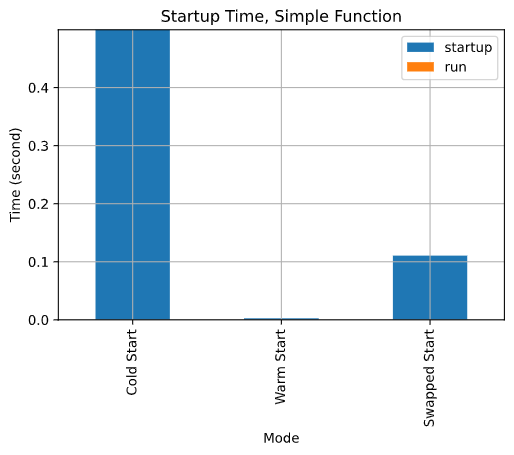
\includegraphics[width=6cm]{http_a.png}
    \caption{Startup time and execution time of a simple function under cold-start, warm-start and swapped-out warm-start.}
    \label{http_a}
\end{figure}
\begin{figure}
    \centering
    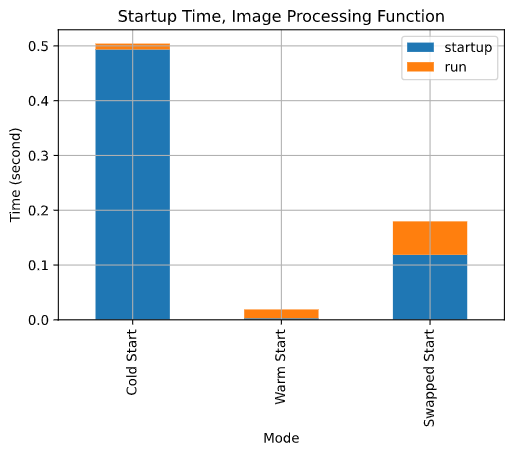
\includegraphics[width=6cm]{image_a.png}
    \caption{Startup time and execution time of an image processing function under cold-start, warm-start and swapped-out warm-start.}
    \label{image_a}
\end{figure}
\begin{figure}
    \centering
    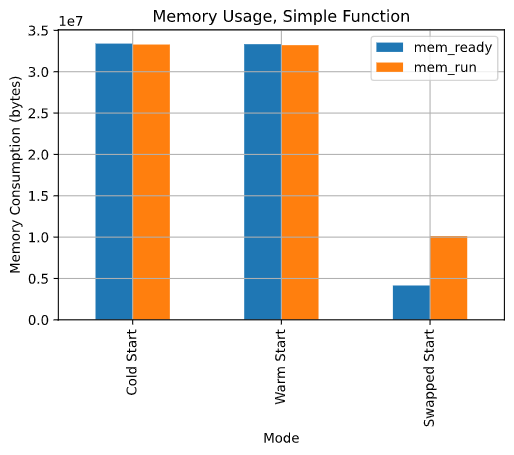
\includegraphics[width=6cm]{http_b.png}
    \caption{Memory consumption of a simple function under cold-start, warm-start and swapped-out warm-start during standby and execution.}
    \label{http_b}
\end{figure}
\begin{figure}
    \centering
    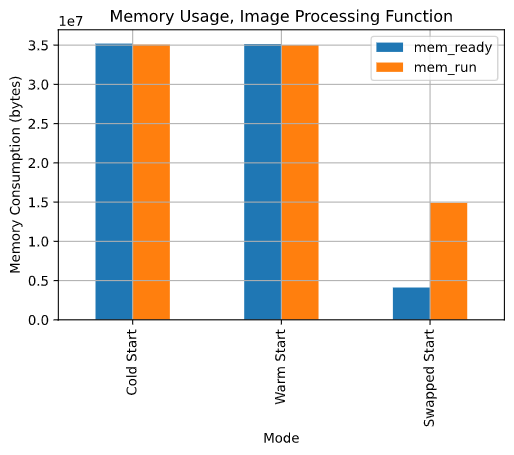
\includegraphics[width=6cm]{image_b.png}
    \caption{Memory consumption of an image processing function under cold-start, warm-start and swapped-out warm-start during standby and execution.}
    \label{image_b}
\end{figure}

\section{Knix Framework Design}

With a promising result from our preliminary tests we proposed to use Knix\cite{akkusSANDHighPerformanceServerless} as a base for our swap trial. Knix is a workflow-based serverless platform, where a workflow is an execution unit and functions are organized in a workflow. In Knix a container is created for each workflow, and each function is executed in a process. This provides the fastest possible cold-start and scale-up time as the creation of new function instance utilizes Linux fork system call to lazy copy another complete and ready instance, skipping both environment and function initialization for new instances. This also further reduce the memory footprint and swap handling time as Linux employs copy-on-write for fork, such that read-only memory content such as the function code and library is not copied, instead shared between forked processes.  

Knix has two level of isolation: container-based isolation between workflows and process-based isolation between function instances. The stronger workflow isolation is for separating workflows possibly of different users. Functions within the same workflow are of the same user, so a weak process-level isolation suffices.

In this section, we first introduce the original organization of Knix. Then, we illustrate how Knix can be modified to utilize swap as a boost method. We then introduces two attempted modification design.

\subsection{Original Design}

In this section, we describe the sandbox section of Knix which is responsible for the deployment of a workflow and all its cooresponding functions. 

\subsubsection{Components}

\paragraph{SandboxAgent}

The SandboxAgent object/process is the entry point of a Knix sandbox. Its main role is to initialize a local queue service, parse workflow and create required FunctionWorker (\ref{functionWorker}), launch the sandbox Frontend (\ref{frontend}), and then the DataLayer. After all initialization of the sandbox is done, the SandboxAgent pulls and handles instructions via global queue service until instructed to shut down.

\paragraph{LocalQueue}\label{localQueue}
The LocalQueue is a service that provides inter-process communication in Knix. A process seeking to use the queue first connects to the LocalQueue via the LocalQueueClient. It can then use the client to create a topic in the queue. Messages can be sent to and pulled from a topic. Messages are modeled as LocalQueueClientMessage objects which consist of a key and a value, which can both be set by the sender.

\paragraph{FunctionWorker}\label{functionWorker}
The FunctionWorker object/process executes a function request. A FunctionWorker is created for each state in the deployed workflow. The FunctionWorker first initializes the runtime environment of the function and retrieves and initializes the function code. Then the FunctionWorker creates and continuously pulls the LocalQueue topic designated by the state to receive requests. Once the FunctionWorker receives a request via the LocalQueue, it forks and create an identical child process to handle the request. The result would first be stored in DataLayer by the key \verb|result_{execution_id}_{function_topic}|, and then be sent via LocalQueue to the next states. The result would also be stored in DataLayer by key \verb|result_{execution_id}| if the current function is the last state. The child process is terminated after handling a request, and the parent FunctionWorker continues to pull LocalQueue for requests while child is processing the request.

\paragraph{Frontend}\label{frontend}
The Frontend is the request entry point process for the workflow. Requests to execute a workflow is sent to the Frontend first. Frontend then put the request to LocalQueue to pass to the topic of the first function. Frontend then waits for the final result appearing in DataLayer, or pulls the Datalayer key upon user requests. Frontend returns the workflow result to the user when available.

\paragraph{DataLayer}\label{dataLayer}
The DataLayer is a shared key-value storage in Knix. Main usage is for result passing and checkpointing. DataLayer service is also open to user function.

\subsubsection{Request flow}

Imagine a request to execute a Knix workflow. The request calls the API endpoint in Frontend. Frontend assigns an execution id, and then pass that to the FunctionWorker of the first state with LocalQueue. FunctionWorker executes its function or state action with forked child, finds out the next state, and then pass the result to the next state with LocalQueue. If the state is an exit state of the workflow, FunctionWorker puts the result on DataLayer instead.  The Frontend is either waiting for the Dataleyer key upon synchronous requests, or pulls the DataLeyer key on user requests upon asynchronous requests. 

\subsection{Design Objectives}
The goal of this modification is to allow Knix to create a large number of ready function instances and have them swapped out to storage. To facilitate this goal, the following objectives should be observed:

\subsubsection{Swapped Instance Pool}
A pool has to be created to manage a large number of function instances. Currently Knix does not have the concept of function instance management as it forks for every function execution and does not reuse instances.

\subsubsection{Pool Scheduling Algorithm}
With an instance pool and the large number of instances, an scheduling algorithm is necessary to determine the action of swapping in or out instances and the creation and deletion of instances based on hardware load and request volume.

\subsubsection{Revised Request Dataflow}
The original Knix structure is highly unmanaged. With a pool of instances, a centralized execution management that follows the progress of each requests and determines the next instance in the workflow facilitate a smooth state transition and pool scheduling and management.

The goal of this modification is to achieve better cold-start latency and a smaller memory footprint.

\subsection{First Design}
\begin{figure}
    \centering
    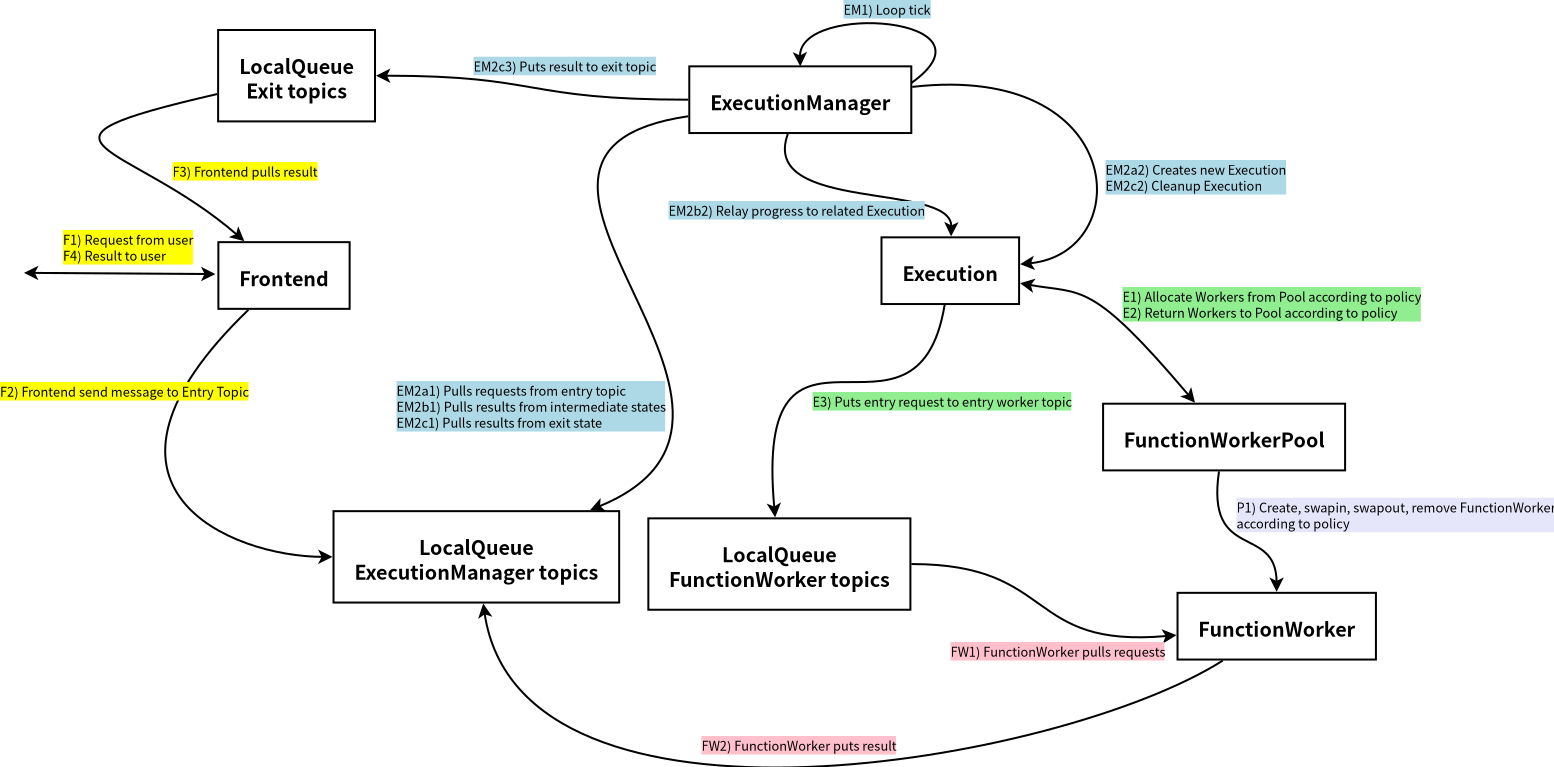
\includegraphics[width=8cm]{knix_new.png}
    \caption{Request dataflow diagram of the first modification.}
    \label{knix_new}
\end{figure}
Fig.\ref{knix_new} shows the structure and dataflow of the first modification. The major addition is the ExecutionManager and the FunctionWorkerPool. The first design code is in the git branch \verb|swap_dev|.

\paragraph{ExecutionManager}
The ExecutionManager service hijacks the original topics FunctionWorker uses to receive requests from Frontend and progresses from FunctionWorker. It creates Execution object for each request. It periodically pulls the function topics for new requests and results from FunctionWorker. Then the requests and results are given to Execution for further process.

\paragraph{Execution}
The Execution object manages the progress and FunctionWorker allocation of a request. Each Execution object comes with an ExecutionPolicy that determines the allocation and return of FunctionWorker instances from the FunctionWorkerPool on new request, on progress or on timer ticks. Execution object also relays requests or results to the appropiate next FunctionWorker instance.

\paragraph{FunctionWorkerPool}
The FunctionWorkerPool handles the creation, swap-in, swap-out and removal of FunctionWorker instances. It has a PoolPolicy that determines the above actions on allocation request, on instance return and on timer ticks.

\paragraph{FunctionWorker}
FunctionWorker is modified such that it now pulls an instance-specific topic on the LocalQueue with topic \verb|{function_topic}_{pid}|. It now does not fork upon request, and handles the request on its own process.

\subsection{Flaws on the first design}
The major flaw of the first design is the very slow deployment and FunctionWorker creation, and the instability comes with it. FunctionWorker is created by FunctionWorkerPool using a new python process each time instead of the original fork, which uses significantly more memory and startup time. The absurd memory usage when FunctionWorkerPool attempts to create a large amount of FunctionWorker on deployment makes the sandbox unstable.

The first design also suspects to a longer request dataflow, potentially prolonging the workflow request latency.

\subsection{Second Design}
The second design returns to a more self-governing approach. The pool management and execution management are combined into the ExecutionManager. The fork method of FunctionWorker spwaning is also being used again. The second design code is in the git branch \verb|swap_impl|.

\paragraph{FunctionWorker}
FunctionWorker is spawned by SandboxAgent. It now also handles fork command which creates a long-living child process. Every FunctionWorker instance reports to ExecutionManager by itself via a single LocalQueue topic \verb|executionManager|. FunctionWorker instances pulls on instance-specific topic \verb|{function_topic}_{pid}|. When it sends its result to the next FunctionWorker, it consults an Execution-instance map living on the DataLayer, and sends the result to appropiate next FunctionWorker instance topic by itself. If the map entry does not contain the next instance information, FunctionWorker waits for it.

\paragraph{ExecutionManager}
ExecutionManager now maintains an Execution-instance map on the DataLayer. The map contains the set of FunctionWorker instance topics of every state of the workflow for a certain request execution id, and also extra sets for new requests. This shared map allows Frontend and FunctionWorker to directly pass requests and results to the correct next instance without ExecutionManager relaying them. The map can be partly filled to adapt to the instance allocation and scheduling. ExecutionManager also handles the work of the previous FunctionWorkerPool when maintaining the mapping.

The new structure should restore the request dataflow to the original, and eliminate the instability issue due to poor instance creation method. However the second design is currently unfinished.

\section{Future Works}
Some area of this project is not finished, including the algorithm for instance scheduling and scaling and performance isolation concerns. 

The instance scheduling algorithm should be able to adjust instance numbers and usage according to workflow progresses and load, in order to provide a service guarantee of the workflow execution. 

There is no performance isolation in current Knix implementation as the FunctionWorker instances are plain processes, which creates uncertainty in maintaining the service guarantee. We hope to provide a lightweight isolation with podman.

The ultimate goal of this project is to provide a serverless platform with balanced cold-start, performance isolation, memory footprint and service guarantee.

\bibliographystyle{IEEEtran}
\bibliography{main}

\end{document}
